\documentclass[12pt,twoside]{article}

\textwidth 17cm \textheight 25cm \evensidemargin 0cm
\oddsidemargin 0cm \topmargin -2cm
\parindent 0pt
%\parskip \bigskipamount

\usepackage{graphicx}
\usepackage[dutch]{babel}
\usepackage{amssymb,amsthm,amsmath}
%\usepackage{dot2texi}
\usepackage[utf8]{inputenc}
\usepackage{nopageno}
\usepackage{pdfpages}
\usepackage{enumerate}
\usepackage{caption}
\usepackage{wrapfig}
\usepackage{pgf,tikz,pgfplots}
\pgfplotsset{compat=1.15}
\usepackage{color}
\usetikzlibrary{arrows}
\usetikzlibrary{patterns}
\usepackage{fancyhdr}
\pagestyle{fancy}
\usepackage[version=3]{mhchem}
\usepackage{multicol}
\usepackage{fix-cm}
\usepackage{setspace}
\usepackage{mhchem}
\usepackage{xhfill}
\usepackage{parskip}
\usepackage{cancel}
\usepackage{mdframed}
\usepackage{url}
\usepackage{mathtools}
\usepackage{changepage}

\newcommand{\todo}[1]{{\color{red} TODO: #1}}

\newcommand{\degree}{\ensuremath{^\circ}}
\newcommand\rad{\qopname\relax o{\mathrm{rad}}}

\newcommand\ggd{\qopname\relax o{\mathrm{ggd}}}

\pgfmathdeclarefunction{gauss}{2}{%
  \pgfmathparse{1/(#2*sqrt(2*pi))*exp(-((x-#1)^2)/(2*#2^2))}%
}

\def\LRA{\Leftrightarrow}

\newcommand{\zrmbox}{\framebox{\phantom{EXE}}\phantom{X}}
\newcommand{\zrm}[1]{\framebox{#1}}

% environment oefening:
% houdt een teller bij die de oefeningen nummert, probeert ook de oefening op één pagina te houden
\newcounter{noefening}
\setcounter{noefening}{0}
\newenvironment{oefening}
{
  \stepcounter{noefening}
  \pagebreak[0]
  \begin{minipage}{\textwidth}
  \vspace*{0.7cm}{\large\bf Oefening \arabic{noefening}}
}{%
  \end{minipage}
}

\usepackage{calc}

% vraag
\reversemarginpar
\newcounter{punten}
\setcounter{punten}{0}
\newcounter{nvraag}
\setcounter{nvraag}{1}
\newlength{\puntwidth}
\newlength{\boxwidth}
\newcommand{\vraag}[1]{
\settowidth{\puntwidth}{\Large{#1}}
\setlength{\boxwidth}{1.5cm}
\addtolength{\boxwidth}{-\puntwidth}
{\large\bf Vraag \arabic{nvraag} \addtocounter{nvraag}{1}}\vspace*{-0.5cm}
{\marginpar{\color{lightgray}\fbox{\parbox{1.5cm}{\vspace*{1cm}\hspace*{\boxwidth}{\Large{#1}}}}}
\vspace*{0.5cm}}
\addtocounter{punten}{#1}}

% arulefill
\def\arulefill{\leavevmode{\xrfill[-5pt]{0.3pt}[lightgray]\endgraf}\vspace*{0.2cm}}

% \arules{n}
\newcommand{\arules}[1]{
\color{lightgray}
%\vspace*{0.05cm}
\foreach \n in {1,...,#1}{
  \vspace*{0.75cm}
  \hrule height 0.3pt\hfill
}\color{black}\vspace*{0.2cm}}

% \arule{x}
\newcommand{\arule}[1]{
\color{lightgray}{\raisebox{-0.1cm}{\rule[-0.05cm]{#1}{0.3pt}}}\color{black}
}

% \abox{y}
\newcommand{\abox}[1]{
\fbox{
\begin{minipage}{\textwidth- 4\fboxsep}
\hspace*{\textwidth}\vspace{#1}
\end{minipage}
}
}

\newcommand{\ruitjes}[1]{
\definecolor{cqcqcq}{rgb}{0.85,0.85,0.85}
\hspace*{-2.5cm}
\begin{tikzpicture}[scale=1.04,line cap=round,line join=round,>=triangle 45,x=1.0cm,y=1.0cm]
\draw [color=cqcqcq, xstep=0.5cm, ystep=0.5cm] (0,-#1) grid (20.5,0);
\end{tikzpicture}
}


\newcommand{\assenstelsel}[5][1]{
\definecolor{cqcqcq}{rgb}{0.65,0.65,0.65}
\begin{tikzpicture}[line cap=round,line join=round,>=triangle 45,x=#1cm,y=#1cm]
\draw [color=cqcqcq,dash pattern=on 1pt off 1pt, xstep=1.0cm,ystep=1.0cm] (#2,#4) grid (#3,#5);
\draw[->,color=black] (#2,0) -- (#3,0);
%\draw[shift={(1,0)},color=black] (0pt,2pt) -- (0pt,-2pt) node[below] {\footnotesize $1$};
%\draw[color=black] (#3.25,0.07) node [anchor=south west] {$x$};
\draw[->,color=black] (0,#4) -- (0,#5);
%\draw[shift={(0,1)},color=black] (2pt,0pt) -- (-2pt,0pt) node[left] {\footnotesize $1$};
\draw[color=black] (0.09,#5.25) node [anchor=west] {\phantom{$y$}};
%\draw[color=black] (0pt,-10pt) node[right] {\footnotesize $0$};
\end{tikzpicture}
}

\newcommand{\getallenas}[3][1]{
\definecolor{cqcqcq}{rgb}{0.65,0.65,0.65}
\begin{tikzpicture}[scale=#1,line cap=round,line join=round,>=triangle 45,x=1.0cm,y=1.0cm]
\draw [color=cqcqcq,dash pattern=on 1pt off 1pt, xstep=1.0cm,ystep=1.0cm] (#2,-0.2) grid (#3,0.2);
\draw[->,color=black] (#2.25,0) -- (#3.5,0);
\draw[shift={(0,0)},color=black] (0pt,2pt) -- (0pt,-2pt) node[below] {\footnotesize $0$};
\draw[shift={(1,0)},color=black] (0pt,2pt) -- (0pt,-2pt) node[below] {\footnotesize $1$};
\draw[color=black] (#3.25,0.07) node [anchor=south west] {$\mathbb{R}$};
\end{tikzpicture}
}

\newcommand{\visgraad}[1]{\begin{tabular}{p{0.5cm}|p{#1}}&\\\hline\\\end{tabular}}

\newcommand{\tekenschema}[2]{\begin{tabular}{p{0.5cm}|p{#1}}&\\\hline\\[#2]\end{tabular}}

% schema van Horner
\newcommand{\schemahorner}{
\begin{tabular}{p{0.5cm}|p{7cm}}
&\\[1.5cm]
\hline\\
\end{tabular}}

% geef tabular iets meer ruimte
\setlength{\tabcolsep}{14pt}
\renewcommand{\arraystretch}{1.5}

\newcommand{\toets}[3]{
\thispagestyle{plain}
\vspace*{-2.5cm}
\begin{tikzpicture}[remember picture, overlay]
    \node [shift={(15.25 cm,-1.6cm)}] {%
        \includegraphics[width=1.8cm]{/home/ppareit/kaa1415/logokaavelgem.png}%
    };%
\end{tikzpicture}

\begin{tabular}{|llc|c|}
\hline
\vspace*{-0.5cm}
&&&\\
Naam & \arule{4cm} & {\Large\bf KA AVELGEM} & \\
\vspace*{-0.75cm}
&&&\\
Klas & \arule{4cm} & {\Large\bf 20...-...-...} & \\
\hline
\vspace*{-0.75cm}
&&&\\
Toets & {\bf #2} & {\large\bf #1} & Beoordeling\\
\vspace*{-0.75cm}
&&&\\
Onderwerp & \multicolumn{2}{l|}{\bf #3} &\\
\hline
\end{tabular}
}

\newcommand{\oefeningen}[1]{

\fancyhead[LE, RO]{\vspace{0.5cm} #1}
%\thispagestyle{plain}

{\bf \Large \centering Oefeningen: #1}

}

\raggedbottom

\newcommand\vl{\qopname\relax o{\mathrm{vl}}}

\newcommand\dom{\qopname\relax o{\mathrm{dom}}}
\newcommand\ber{\qopname\relax o{\mathrm{ber}}}

\newcommand\mC{\qopname\relax o{\mathrm{mC}}}
\newcommand\uC{\qopname\relax o{\mathrm{{\mu}C}}}
\newcommand\C{\qopname\relax o{\mathrm{C}}}

\newcommand\W{\qopname\relax o{\mathrm{W}}}
\newcommand\kW{\qopname\relax o{\mathrm{kW}}}
\newcommand\kWh{\qopname\relax o{\mathrm{kWh}}}


\newcommand\V{\qopname\relax o{\mathrm{V}}}
\newcommand\ohm{\qopname\relax o{\mathrm{\Omega}}}
\newcommand\kohm{\qopname\relax o{\mathrm{k\Omega}}}


\newcommand\N{\qopname\relax o{\mathrm{N}}}

\newcommand\Nperkg{\qopname\relax o{\mathrm{N/kg}}}

\newcommand\Nperm{\qopname\relax o{\mathrm{N/m}}}

\newcommand\gpermol{\qopname\relax o{\mathrm{g/mol}}}


\newcommand\kgperm{\qopname\relax o{\mathrm{kg/m}}}
\newcommand\kgperdm{\qopname\relax o{\mathrm{kg/dm}}}
\newcommand\gpercm{\qopname\relax o{\mathrm{g/cm}}}
\newcommand\gperml{\qopname\relax o{\mathrm{g/ml}}}


\newcommand{\mA}{\;\mbox{mA}}
\newcommand{\A}{\;\mbox{A}}
\newcommand{\MA}{\;\mbox{MA}}

\newcommand{\us}{\;\mu\mbox{s}}
\newcommand\s{\qopname\relax o{\mathrm{s}}}

\newcommand\h{\qopname\relax o{\mathrm{h}}}

\newcommand{\kmperh}{\;\mbox{km/h}}
\newcommand{\mpers}{\;\mbox{m/s}}
\newcommand{\kmpermin}{\;\mbox{km/min}}
\newcommand{\kmpers}{\;\mbox{km/s}}

\newcommand{\mph}{\;\mbox{mph}}

\newcommand{\Hz}{\;\mbox{Hz}}

\newcommand\Gm{\qopname\relax o{\mathrm{Gm}}}
\newcommand\Mm{\qopname\relax o{\mathrm{Mm}}}
\newcommand\km{\qopname\relax o{\mathrm{km}}}
\newcommand\hm{\qopname\relax o{\mathrm{hm}}}
\newcommand\dam{\qopname\relax o{\mathrm{dam}}}
\newcommand\m{\qopname\relax o{\mathrm{m}}}
\newcommand\dm{\qopname\relax o{\mathrm{dm}}}
\newcommand\cm{\qopname\relax o{\mathrm{cm}}}
\newcommand\mm{\qopname\relax o{\mathrm{mm}}}
\newcommand\um{\qopname\relax o{\mathrm{{\mu}m}}}
\newcommand\nm{\qopname\relax o{\mathrm{nm}}}


\newcommand\Gg{\qopname\relax o{\mathrm{Gg}}}
\newcommand\Mg{\qopname\relax o{\mathrm{Mg}}}
\newcommand\kg{\qopname\relax o{\mathrm{kg}}}
\newcommand\hg{\qopname\relax o{\mathrm{hg}}}
\renewcommand\dag{\qopname\relax o{\mathrm{dag}}}
\newcommand\g{\qopname\relax o{\mathrm{g}}}
\newcommand\dg{\qopname\relax o{\mathrm{dg}}}
\newcommand\cg{\qopname\relax o{\mathrm{cg}}}
\newcommand\mg{\qopname\relax o{\mathrm{mg}}}
\newcommand\ug{\qopname\relax o{\mathrm{{\mu}g}}}
\renewcommand\ng{\qopname\relax o{\mathrm{ng}}}

\newcommand\ton{\qopname\relax o{\mathrm{ton}}}

\newcommand\Gl{\qopname\relax o{\mathrm{Gl}}}
\newcommand\Ml{\qopname\relax o{\mathrm{Ml}}}
\newcommand\kl{\qopname\relax o{\mathrm{kl}}}
\newcommand\hl{\qopname\relax o{\mathrm{hl}}}
\newcommand\dal{\qopname\relax o{\mathrm{dal}}}
\renewcommand\l{\qopname\relax o{\mathrm{l}}}
\newcommand\dl{\qopname\relax o{\mathrm{dl}}}
\newcommand\cl{\qopname\relax o{\mathrm{cl}}}
\newcommand\ml{\qopname\relax o{\mathrm{ml}}}
\newcommand\ul{\qopname\relax o{\mathrm{{\mu}l}}}
\newcommand\nl{\qopname\relax o{\mathrm{nl}}}

\newcommand\MJ{\qopname\relax o{\mathrm{MJ}}}
\newcommand\kJ{\qopname\relax o{\mathrm{kJ}}}
\newcommand\J{\qopname\relax o{\mathrm{J}}}

\newcommand\T{\qopname\relax o{\mathrm{T}}}
\newcommand\uT{\qopname\relax o{\mathrm{{\mu}T}}}

\newcommand\grC{\qopname\relax o{\mathrm{{\degree}C}}}

\newcommand\K{\qopname\relax o{\mathrm{K}}}
\newcommand\calperK{\qopname\relax o{\mathrm{cal/K}}}

\newcommand\hPa{\qopname\relax o{\mathrm{hPa}}}
\newcommand\Pa{\qopname\relax o{\mathrm{Pa}}}

\newcommand\dB{\qopname\relax o{\mathrm{dB}}}

\newcommand\Var{\qopname\relax o{\mathrm{Var}}}

\newcommand{\EE}[1]{\cdot 10^{#1}}

\onehalfspacing

%\setlength{\headsep}{0cm}

\newenvironment{exlist}[1] %
{ \begin{multicols}{#1}
  \begin{enumerate}[(a)]
    \setlength{\itemsep}{0.5em} }
{ \end{enumerate}
  \end{multicols} }




\usepackage{pgfplots}

\usepackage{relsize}

\begin{document}

\thispagestyle{empty}
\begin{center}
  \begin{mdframed}
  \centering
  \fontsize{40}{60}\selectfont Logaritmische functies
  \end{mdframed}
  \vfill
  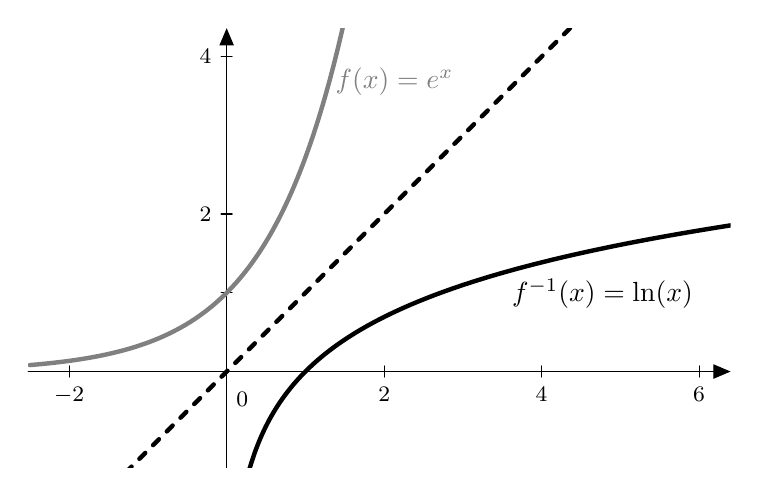
\begin{tikzpicture}[line cap=round,line join=round,>=triangle 45,x=1.0cm,y=1.0cm]
  \draw[->,color=black] (-2.52,0) -- (6.4,0);
  \foreach \x in {-2,2,4,6}
  \draw[shift={(\x,0)},color=black] (0pt,2pt) -- (0pt,-2pt) node[below] {\footnotesize $\x$};
  \draw[->,color=black] (0,-1.22) -- (0,4.36);
  \foreach \y in {,2,4}
  \draw[shift={(0,\y)},color=black] (2pt,0pt) -- (-2pt,0pt) node[left] {\footnotesize $\y$};
  \draw[color=black] (0pt,-10pt) node[right] {\footnotesize $0$};
  \clip(-2.52,-1.22) rectangle (6.4,4.36);
  \draw[line width=1.6pt,dash pattern=on 3pt off 4pt, smooth,samples=50,domain=-2.5:6.4] plot(\x,{(\x)});
  \draw[color=gray,line width=1.6pt, smooth,samples=100,domain=-2.5:2.4] plot(\x,{exp(\x)});
  \draw[line width=1.6pt, smooth,samples=100,domain=0.1:6.4] plot(\x,{ln((\x))});
  \draw[color=gray] (1.26,3.98) node[anchor=north west] {$f(x)=e^x$};
  \draw (3.5,1.3) node[anchor=north west] {$f^{-1}(x)=\ln(x)$};
  \end{tikzpicture}
  \vfill
\end{center}

\subsection*{Doelstellingen}
\vspace*{-0.8cm}
{\singlespacing
Je \hfill  {\scriptsize(LP2006-059, LI1.8, ET23,14,32,25,31,24)}
\begin{itemize}
  \itemsep-0.2em
  \item kent de definitie van een logaritme met een willekeurig grondtal;
  \item kan de onderstaande rekenregels toepassen: (U)
  \begin{itemize}
    \item logaritme van een product,
    \item logaritme van een quotiënt,
    \item logaritme van een macht,
    \item verandering van grondtal;
  \end{itemize}
  \item kent de logaritmische functie $f( x ) = \log_a x$ als inverse van de exponentiële functie $f( x ) = a^x$;
  \item kan domein, bereik, bijzondere waarden, tekenverloop, stijgen\&dalen en asymptotisch gedrag bepalen van logaritmische functies;
  \item kent de begrippen beginwaarde, groeifactor, groeipercentage, halveringstijd en verdubbelingstijd;
  \item kan vraagstukken en problemen oplossen die aanleiding geven tot een exponentiële vergelijking of functie;
  \item kan uit de betrekking $a^b = c$ de derde veranderlijke berekenen als de twee andere gegeven zijn.
\end{itemize}}

\thispagestyle{empty}
\mbox{}
\newpage
\clearpage
\thispagestyle{empty}
%\mbox{}
\tableofcontents
\newpage
\clearpage
\pagenumbering{arabic} 

\fancyhead[RO,LE]{Logaritmische functies}
\fancyhead[RE,LO]{}


\section{Definitie}

\paragraph{Logaritme}
\begin{mdframed}
De {\bf logaritme met grondtal $a$} ($a\in\mathbb{R}\backslash\{0,1\}$) van een reëel getal $x$ is de exponent
waartoe we a moeten verheffen om dit getal te bekomen:
$$\log_a x = y \Leftrightarrow a^y=x$$
\end{mdframed}

Een logaritme zoeken is dus een exponent zoeken!

\paragraph{Voorbeelden}
\begin{enumerate}[(a)]
  \item $\log_3 9 = 2$ want $3^2=9$
  \item $\log_5\sqrt{125} = ?$
  \begin{eqnarray*}
    \log_5\sqrt{125}=y &\LRA& \sqrt{125} = 5^y\\
                       &\LRA& 125^\frac{1}{2} = 5^y\\
                       &\LRA& (5^3)^\frac{1}{2} = 5^y\\
                       &\LRA& 5^\frac{3}{2} = 5^y\\
                       &\LRA& y=\frac{3}{2}
  \end{eqnarray*}
  Dus $\log_5\sqrt{125} = \dfrac{3}{2}$
\end{enumerate}

\begin{oefening} % from mathcentre logarithms 2009
Herschrijf met behulp van logaritmen i.p.v. met machten.
\begin{multicols}{4}
\begin{enumerate}[(a)]
  \item $8^2=64$
  \item $10^6=1000000$
  \item $5^{-1}=\dfrac{1}{5}$
  \item $3^5=243$
  \item $10^{-3}=0.001$
  \item $\sqrt{49}=7$
  \item $2^{10}=1024$
  \item $3^{-2}=\dfrac{1}{9}$
  \item $27^{2/3}=9$
  \item $5^3=125$
  \item $6^0=1$
  \item $32^{-2/5}=\dfrac{1}{4}$
\end{enumerate}
\end{multicols}
\end{oefening}

\begin{oefening}
Zoek de logaritme met grondtal $a$ van de volgende getallen:
\begin{multicols}{2}
\begin{enumerate}[(a)]
  \itemsep0.7em
  \item $\log_2 16$
  \item $\log_3 81$
  \item $\log_2 8$
  \item $\log_{10} 10000$
  \item $\log_3 \dfrac{1}{9}$
  \item $\log_e \sqrt{e}$
\end{enumerate}
\end{multicols}
\end{oefening}


\pagebreak
\paragraph{Gevolgen}
\begin{itemize}
  \item Nul en strikt negatieve getallen hebben geen logaritme
  \item Uit $\log_a x = y \Leftrightarrow a^y=x$ volgt
  \begin{mdframed}
  $$\log_a a^y=y$$
  \end{mdframed}
  Dit zie je in door in de eerste gelijkheid $x$ te vervangen door $a^y$.
  \item Ook volgt $x=a^{\log_a x}$ door $y$ in de tweede gelijkheid door $\log_a x$ te vervangen.
  \item Als $y=0$ dan hebben we $\log_a a^0=0$ en dus
  \begin{mdframed}
  $$\log_a 1=0$$
  \end{mdframed}
  \item Als $y=1$ dan hebben we $\log_a a^1=1$ en dus
  \begin{mdframed}
  $$\log_a a=1$$
  \end{mdframed}
\end{itemize}

\begin{oefening} % from mathcentre logarithms 2009
Bepaal de waarde van de volgende logaritmen.
\begin{multicols}{4}
\begin{enumerate}[(a)]
  \item $\log_3 9$
  \item $\log_4 64$
  \item $\log_3 \dfrac{1}{27}$
  \item $\log_a a^5$
  \item $\log_2 32$
  \item $\log_25 5$
  \item $\log_7 1$
  \item $\log_c \sqrt{c}$
  \item $\log_5 125$
  \item $\log_8 2$
  \item $\log_8 \dfrac{1}{8}$
  \item $\log_s s$
  \item $\log_{10} 10000$
  \item $\log_{81} 8$
  \item $\log_4 8$
  \item $\log_e \dfrac{1}{e^3}$
\end{enumerate}
\end{multicols}
\end{oefening}

\begin{oefening}
Bereken:
\begin{exlist}{3}
  \item $\log_2 \sqrt{2}$
  \item $\log_9 \sqrt[5]{9}$
  \item $\log \sqrt{10}$
  \item $\log_4 0.5$
  \item $\log_{\frac{1}{5}} 0.2$
  \item $\ln \dfrac{1}{e\sqrt{e}}$
\end{exlist}
\end{oefening}

\pagebreak
\section{Bijzondere logaritmen}

\subsection{Briggse logaritmen}

Is het grondtal $a$ gelijk aan 10 dan spreken we van {\bf Briggse logaritmen}.

De Engelse wiskundige Henry Briggs publiceerde in 1617 een tafel met deze naar hem genoemde logaritmen.

\paragraph{Notatie} $\log x = \log_{10} x$

\paragraph{Voorbeelden}\begin{minipage}[t]{\textwidth}
\begin{enumerate}[(a)]
  \item $\log 10 = 1$
  \item $\log 1 = 0$
  \item $\log 0.0001 = \log 10^{-4} = -4$
\end{enumerate}
\end{minipage}

\paragraph{Rekenmachine} We kunnen de Briggse logaritmen berekenen op het \zrm{ZRM} met de toets \zrm{log}. Zo is $\log 3459 = 3.5389506$

\subsection{Neperiaanse logaritmen}

Is het grondtal $a$ gelijk aan $e$ dan spreken we van {\bf natuurlijke logaritmen} of Neperiaanse logaritmen, naar de Engelse wiskundige John Napier (1550-1617).

\paragraph{Notatie} $\ln x = \log_{e} x$

\paragraph{Voorbeelden}\begin{minipage}[t]{\textwidth}
\begin{enumerate}[(a)]
  \item $\ln e = 1$
  \item $\ln 1 = 0$
  \item $\ln e^{-2} = -2$
\end{enumerate}
\end{minipage}

\paragraph{Rekenmachine} Natuurlijke logaritmen kunnen op de zakrekenmachine met de \zrm{ln} toets worden berekend.
Zo is $\ln 3459 = 8.1487348$

\begin{oefening}
Bereken met je \zrm{ZRM}, noteer je resultaat met 3 decimalen nauwkeurig.
\begin{multicols}{3}
\begin{enumerate}[(a)]
  \item $\log 12345$
  \item $\log 98.76$
  \item $\log 1.111$
  \item $\ln 12345$
  \item $\ln 98.76$
  \item $\ln 1.111$
\end{enumerate}
\end{multicols}
\end{oefening}

\pagebreak

\section{Rekenregels}

\subsection{Rekenregels van logaritmen met grondtal $a$}

%\paragraph*{Rekenregels van logaritmen met grondtal $a$}
\begin{mdframed}
$\forall x,y \in \mathbb{R}_0^+, \forall p\in \mathbb{R}:$
\begin{align*}
\log_a(x\cdot y) &= \log_a x + \log_a y && \mbox{logaritme van een product}\\
\log_a \dfrac{x}{y} &= \log_a x - \log_a y && \mbox{logaritme van een quotiënt}\\
\log_a \dfrac{1}{y} &= - \log_a y && \mbox{logaritme van een invers}\\
\log_a(x^p) &= p\cdot\log_a x && \mbox{logaritme van een macht}
\end{align*}
\end{mdframed}

\paragraph{Bewijs} Logaritme van een product
\begin{eqnarray*}
  \log_a(x\cdot y) &=& \log_a\left(a^{\log_a x}\cdot a^{\log_a y}\right)\\
                   &=& \log_a\left(a^{\log_a x + \log_a y}\right)\\
                   &=& \log_a x + \log_a y
\end{eqnarray*}

\begin{oefening}
Bewijs de andere rekenregels.
\end{oefening}

\begin{oefening} % argument
Pas de eigenschappen voor de logaritme van een product, quotiënt en macht toe.
\begin{exlist}{3}
  \item $\log \left(x^2y\right)$
  \item $\log \left(x\sqrt{y}\right)$
  \item $\log \left(\dfrac{x\cdot y}{z^2}\right)$
  \item $\log \left(\dfrac{100}{x}\right)$
  \item $\log \left(\dfrac{1}{10}x^2y^3\right)$
  \item $\log_2 \left(8x\sqrt{z}\right)$
  \item $\log \left(2\cdot 10^{-2x}\right)$
  \item $\log \left(5.1\cdot 10^{7x}\right)$
  \item $\ln \left(5\cdot e^{3x}\right)$
\end{exlist}
\end{oefening}

\begin{oefening} % argument
Schrijf als één logaritme.
\begin{exlist}{2}
  \item $2\log x + 5 \log y$
  \item $\log x - 3 \log y$
  \item $\dfrac{1}{2}\log x + 2 \log y$
  \item $\log 7 + x \log 5$
\end{exlist}
\end{oefening}

\begin{oefening} % argument
Bereken zonder \zrm{ZRM}.
\begin{exlist}{2}
  \item $\log_5 10 + \log_5 15 - \log_5 6$
  \item $2\log_2 5 - \log_2 50$
  \item $\log_2 135 - \log_2 18 - \log_2 6 - \log_2 10$
  \item $\log_3 270 - \log_3 12 + 2\log_3 6 - \log_3 30$
\end{exlist}
\end{oefening}

\begin{oefening} % from mathcentre logarithms 2009
Elk van de volgende uitdrukkingen kan herschreven worden als $\log N$. Bepaal de $N$ voor elke uitdrukking. Er wordt dus niet gevraagd om de logaritme uit te rekenen, wel om deze korter te herschrijven.
\begin{exlist}{2}
  \item $\log 3 + \log 5$
  \item $2\log 3 - 3\log 2$
  \item $5\log 2 + 2\log 5$
  \item $\log 12 - 2\log 2 + \log 3$
  \item $\log 16 - \log 2$
  \item $\log 236 - 7\log 2$
  \item $\log 128 - 7\log 2$
  \item $5\log 2 + 4\log 3 - 3\log 4$
  \item $3\log 4$
  \item $\log 236 - \log 1$
  \item $\log 2 + \log 3 + \log 4$
  \item $\log 10 + 2\log 3 - \log 2$
\end{exlist}
\end{oefening}

\begin{oefening} % argument
Zoek $x$.
\begin{exlist}{2}
  \item $\log x + \log 4x = 2$
  \item $2\log_2 x + \log_2 8x = -3$
\end{exlist}
\end{oefening}

\begin{oefening} % argument
Bepaal het grondtal $a$.
\begin{exlist}{2}
  \item $\log_a 2 + \log_a 8 = 4$
  \item $\log_a 16 = 2\cdot \log_4 16$
  \item $\log_a 3 + \log_a 27 = 4$
  \item $2 \log_a 2 - \log_a 3 + \dfrac{2}{3}\log_a 27 = 2$  
\end{exlist}
\end{oefening}

\pagebreak
\subsection{Veranderen van grondtal}

\begin{mdframed}
$\forall a,b,c \in \mathbb{R}_0^+\backslash\{1\}:$
\begin{align*}
\log_b x &= \dfrac{\log_a x}{\log_a b} && \mbox{veranderen van grondtal}\\
\log_b x &= \dfrac{1}{\log_x b} && \mbox{omwisseling grondtal en argument}
\end{align*}
\end{mdframed}

\paragraph*{Voorbeelden}
\begin{itemize}
  \item Ons \zrm{ZRM} bevat enkel de toetsen \zrm{log} en \zrm{ln}. Dus steeds als we een logaritme met een willekeurig grondtal verschillend van $10$ of $e$ willen berekenen moeten we veranderen van grondtal, bijvoorbeeld:
  \begin{align*}
    \log_{7}343 &= \dfrac{\log 452}{\log 7}\\
                &\approx 3.14 \qquad\mbox{met \zrm{ZRM}} 
  \end{align*}
  \item Soms kunnen we logaritmen berekenen die anders moeilijk rechtstreeks in het gegeven grondtal te berekenen zijn, bijvoorbeeld:
  \begin{align*}
    \log_{8}32 &= \dfrac{\log_2 32}{\log_2 8}\\
               &= \dfrac{5}{3} 
  \end{align*}
  \item En als het grondtal en argument op de foute plaats staan om makkelijk een logaritme te bereken, dan kunnen we ze als volgt wisselen:
  \begin{align*}
    \log_{16}2 &= \dfrac{1}{\log_2 16}\\
               &= \dfrac{1}{4}
  \end{align*}
\end{itemize}


\begin{oefening} % argument
Bereken zonder \zrm{ZRM}
\begin{exlist}{2}
  \item $\log_2 7 \cdot \log_7 16$
  \item $\log 11 \cdot \log_{11} 0.1$
  \item $\log_9 27$
  \item $\log_{32} 64$
  \item $\dfrac{\ln 81}{\ln 3}$
  \item $\dfrac{\ln 81}{\ln 27}$
  \item $\log_8 27 \cdot \log_3 8$
  \item $\ln 4 \cdot \log_4 (\sqrt{e}\cdot e^2)$
  \item $\dfrac{1}{\log_8 2}$
  \item $\log_27 3$
  \item $\dfrac{\log_8 125}{\log_8 5}$
  \item $\log_8 16$
\end{exlist}
\end{oefening}

\begin{oefening} % from mathcentre logarithms 2009
Gebruik logaritmen om de volgende vergelijkingen op te lossen. Geef de oplossingen in decimale notatie met 3 cijfers na de komma. Geef steeds de oplossingenverzameling en maak steeds de proef.
\begin{exlist}{2}
  \item $10^x=5$
  \item $4^x=12$
  \item $\pi^x=10$
  \item $e^x=8$
  \item $3^x=2$
  \item $e^x=\pi$
  \item $10^x=\dfrac{1}{2}$
  \item $7^x=1$
  \item $\left(\dfrac{1}{3}\right)^x=2$
  \item $e^x=0.1$
  \item $\left(\dfrac{1}{2}\right)^x=\dfrac{1}{100}$
  \item $10^x=e^{2x-1}$
\end{exlist}
\end{oefening}


\pagebreak
\section{Logaritmische functie}

\subsection{Definitie}
De reële functie die elk reëel getal afbeeldt op zijn logaritme met grondtal $a$ noemen we de {\bf logaritmische functie met grondtal $a$}:
$$f(x) = \log_a x$$

\subsection{Hoofdeigenschap}

\begin{mdframed}
De logaritmische functie met grondtal $a$ en de exponentiële functie met grondtal $a$ zijn inverse functies.
\end{mdframed}

\paragraph{Voorbeeld} $y=\log_2 x$ en $y=2^x$

\subsection{Gevolgen}

\begin{multicols}{2}
  \begin{center}
  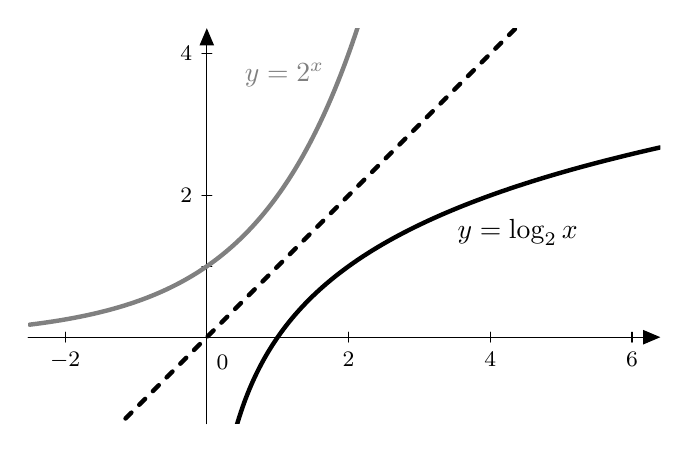
\begin{tikzpicture}[scale=0.9,line cap=round,line join=round,>=triangle 45,x=1.0cm,y=1.0cm]
    \draw[->,color=black] (-2.52,0) -- (6.4,0);
    \foreach \x in {-2,2,4,6}
    \draw[shift={(\x,0)},color=black] (0pt,2pt) -- (0pt,-2pt) node[below] {\footnotesize $\x$};
    \draw[->,color=black] (0,-1.22) -- (0,4.36);
    \foreach \y in {,2,4}
    \draw[shift={(0,\y)},color=black] (2pt,0pt) -- (-2pt,0pt) node[left] {\footnotesize $\y$};
    \draw[color=black] (0pt,-10pt) node[right] {\footnotesize $0$};
    \clip(-2.52,-1.22) rectangle (6.4,4.36);
    \draw[line width=1.6pt,dash pattern=on 3pt off 4pt, smooth,samples=50,domain=-2.5:6.4] plot(\x,{(\x)});
    \draw[color=gray,line width=1.6pt, smooth,samples=100,domain=-2.5:2.4] plot(\x,{exp(ln(2)*\x)});
    \draw[line width=1.6pt, smooth,samples=100,domain=0.1:6.4] plot(\x,{ln((\x))/ln(2)});
    \draw[color=gray] (0.4,4) node[anchor=north west] {$y=2^x$};
    \draw (3.4,1.8) node[anchor=north west] {$y=\log_2 x$};
  \end{tikzpicture}
  \end{center}
  \begin{center}
  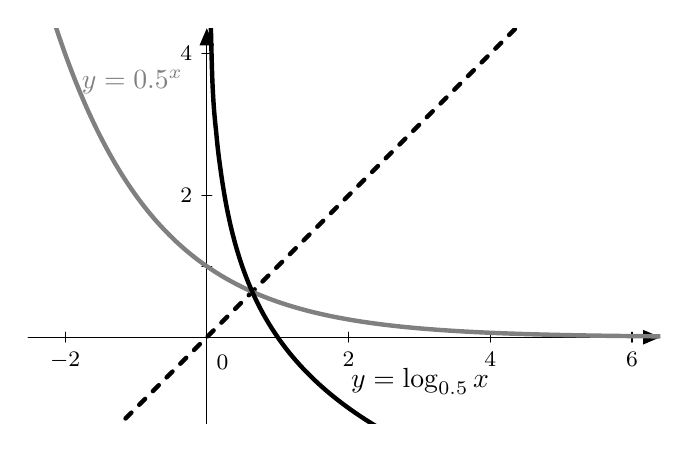
\begin{tikzpicture}[scale=0.9,line cap=round,line join=round,>=triangle 45,x=1.0cm,y=1.0cm]
    \draw[->,color=black] (-2.52,0) -- (6.4,0);
    \foreach \x in {-2,2,4,6}
    \draw[shift={(\x,0)},color=black] (0pt,2pt) -- (0pt,-2pt) node[below] {\footnotesize $\x$};
    \draw[->,color=black] (0,-1.22) -- (0,4.36);
    \foreach \y in {,2,4}
    \draw[shift={(0,\y)},color=black] (2pt,0pt) -- (-2pt,0pt) node[left] {\footnotesize $\y$};
    \draw[color=black] (0pt,-10pt) node[right] {\footnotesize $0$};
    \clip(-2.52,-1.22) rectangle (6.4,4.36);
    \draw[line width=1.6pt,dash pattern=on 3pt off 4pt, smooth,samples=50,domain=-2.5:6.4] plot(\x,{(\x)});
    \draw[color=gray,line width=1.6pt, smooth,samples=100,domain=-2.5:6.4] plot(\x,{exp(ln(0.5)*\x)});
    \draw[line width=1.6pt, smooth,samples=100,domain=0.01:6.4] plot(\x,{ln((\x))/ln(0.5)});
    \draw[color=gray] (-1.9,3.9) node[anchor=north west] {$y=0.5^x$};
    \draw (1.9,-0.3) node[anchor=north west] {$y=\log_{0.5} x$};
  \end{tikzpicture}
  \end{center}
\end{multicols}

\begin{itemize}
  \item De grafieken van de logaritmische en exponentiële functies zijn elkaars spiegelbeeld ten opzichte van de eerste bissectrice in een orthonormaal assenstelsel.
  \item $\dom \log_a x = \mathbb{R}^+_0$ en $\ber \log_a x = \mathbb{R}$
  \item Bijzondere punten: $(1, 0)$ en $(a, 1)$\\
\end{itemize}
  \begin{minipage}{0.5\textwidth}
    \centering $a>1$
    \begin{itemize}
      \item $\log_a x$ is stijgend in $\mathbb{R}^+_0$
      \item $\lim_{+\infty} \log_a x = +\infty$
      \item $\lim_{x\underset{>}{\to}0} \log_a x = -\infty$
    \end{itemize}
  \end{minipage}\vline
  \begin{minipage}{0.5\textwidth}
    \centering $0<a<1$
    \begin{itemize}
      \item $\log_a x$ is dalend in $\mathbb{R}^+_0$
      \item $\lim_{+\infty} \log_a x = -\infty$
      \item $\lim_{x\underset{>}{\to}0} \log_a x = +\infty$
    \end{itemize}
  \end{minipage}
  \begin{itemize}
    \item De $y$-as met vergelijking $x=0$ is een verticale asymptoot.
  \end{itemize}

\begin{oefening}
Teken op éénzelfde assenstelsel de functies
$$f(x)=e^x\qquad g(x)=\ln(x)$$
\begin{enumerate}[(a)]
  \item Via welke transformatie kunnen we van $f$ naar $g$ gaan?
  \item Teken deze transformatie ook op het assenstelsel.
  \item Hoe noemen we twee functies die dit verband hebben?
  \item Toon dit ook algebraïsch aan.
\end{enumerate}
\end{oefening}

\begin{oefening} % argument, modified
Maak de grafiek van de logaritmische functie met voorschrift:
\begin{exlist}{3}
  \item $f(x)=\log_2 x$
  \item $f(x)=\log_{0.5}x$
  \item $f(x)=\ln x$
  \item $f(x)=3+\log_2 x$
  \item $f(x)=\log_2(x-3)$
  \item $f(x)=3\log_2 x$
\end{exlist}
\end{oefening}

\begin{oefening}
Hieronder vind je de grafiek van een logaritmische functie met voorschrift $f(x)=\log_a x$. Lees $a$ op de figuur af.
\begin{exlist}{2}
  \item
  \begin{center}
\definecolor{cqcqcq}{rgb}{0.75,0.75,0.75}
\begin{tikzpicture}[line cap=round,line join=round,>=triangle 45,x=1.0cm,y=1.0cm]
\draw [color=cqcqcq,dash pattern=on 1pt off 1pt, xstep=0.5cm,ystep=0.5cm] (-0.5,-0.5) grid (5.5,5.5);
\draw[->,color=black] (-0.5,0) -- (5.5,0);
\foreach \x in {1,2,3,4,5}
\draw[shift={(\x,0)},color=black] (0pt,2pt) -- (0pt,-2pt) node[below] {\footnotesize $\x$};
\draw[->,color=black] (0,-0.5) -- (0,5.5);
\foreach \y in {1,2,3,4,5}
\draw[shift={(0,\y)},color=black] (2pt,0pt) -- (-2pt,0pt) node[left] {\footnotesize $\y$};
\draw[color=black] (0pt,-10pt) node[right] {\footnotesize $0$};
\clip(-0.5,-0.5) rectangle (5.5,5.5);
\draw[line width=1.6,smooth,samples=100,domain=0.01:5.5] plot(\x,{ln((\x))/ln(1.5)});
\end{tikzpicture}
  \end{center}
  \item
  \begin{center}
\definecolor{cqcqcq}{rgb}{0.75,0.75,0.75}
\begin{tikzpicture}[line cap=round,line join=round,>=triangle 45,x=1.0cm,y=1.0cm]
\draw [color=cqcqcq,dash pattern=on 1pt off 1pt, xstep=0.5cm,ystep=0.5cm] (-0.5,-0.5) grid (5.5,5.5);
\draw[->,color=black] (-0.5,0) -- (5.5,0);
\foreach \x in {1,2,3,4,5}
\draw[shift={(\x,0)},color=black] (0pt,2pt) -- (0pt,-2pt) node[below] {\footnotesize $\x$};
\draw[->,color=black] (0,-0.5) -- (0,5.5);
\foreach \y in {1,2,3,4,5}
\draw[shift={(0,\y)},color=black] (2pt,0pt) -- (-2pt,0pt) node[left] {\footnotesize $\y$};
\draw[color=black] (0pt,-10pt) node[right] {\footnotesize $0$};
\clip(-0.5,-0.5) rectangle (5.5,5.5);
\draw[line width=1.6,smooth,samples=100,domain=0.01:5.5] plot(\x,{ln((\x))/ln(0.75)});
\end{tikzpicture}
  \end{center}
\end{exlist}
\end{oefening}

\begin{oefening} % argument, modified
Bepaal:
\begin{exlist}{3}
  \item $\displaystyle\lim_{x\to +\infty}\log_5 x$
  \item $\displaystyle\lim_{x\to +\infty}\log_{0.3} x$
  \item $\displaystyle\lim_{x\underset{>}{\to} 0}\log_4 x$
  \item $\displaystyle\lim_{x\underset{>}{\to} 0}\log_{0.4} x$
  \item $\displaystyle\lim_{x\to +\infty}\log_{1.01} x$
  \item $\displaystyle\lim_{x\to +\infty}\log_{0.99} x$
  \item $\displaystyle\lim_{x\to +\infty}\log_{3} (8x)$
  \item $\displaystyle\lim_{x\underset{>}{\to} 0}\log_{2} x$
  \item $\displaystyle\lim_{x\underset{<}{\to} 0}\log (-x)$
\end{exlist}
\end{oefening}

\begin{oefening} % argument, modified
Een functie met voorschrift $f(x)=\log_a kx$ gaat door $P(2,1)$ en door $Q(4,\dfrac{3}{2})$. Bepaal $a$ en $k$.
\end{oefening}

\section{Toepassingen}

\begin{oefening} % argument, modified
Een blauwe plek heelt exponentieel. Als $S_0$ de oorspronkelijke oppervlakte is, dan is de oppervlakte $S$ na $t$ dagen:
$$S_t=S_0e^{-0.35\cdot t}$$
\begin{enumerate}[(a)]
  \item Hoeveel percent blijft er over na 10 dagen?
  \item Na hoeveel dagen is de helft van de blauwe plek geheeld?
\end{enumerate}
\end{oefening}

\vspace*{-0.5cm}

\begin{oefening}
Op het tijdstip $t=0$ bevat een bacteriën kolonie 400 bacteriën. Elk uur groeit het aantal aan met $5 \%$. We vonden de formule voor het aantal $N$ na $t$ uur:
$$N=400\cdot 1.05^t\;.$$
Na hoeveel uur is het aantal bacteriën verdubbeld?
\end{oefening}

\begin{oefening}
Een patiënt wordt voor een operatie onder narcose gebracht door $1200 \mg$ van een verdovingsmiddel in te spuiten. De nieren zorgen er echter voor dat die hoeveelheid ieder uur vermindert met $26 \%$. Tijdens de operatie is een minimum van $500 \mg$ vereist. Hoelang mag de operatie duren?
\end{oefening}

\begin{oefening}
Een satelliet heeft een elektriciteitsvoorziening met een vermogen van
$$P=120\cdot e^{-0.004\cdot t}\;.$$
Daarin is $P$ uitgedrukt in watt en is $t$ het aantal dagen na de lancering.
\begin{enumerate}[(a)]
  \item Hoeveel watt is er nog beschikbaar na $1$ jaar?
  \item Voor de werking van de satelliet is een minimaal vermogen van 10 watt nodig. Bereken de levensduur van de satelliet.
\end{enumerate}
\end{oefening}

\begin{oefening}
Als je geld belegt, dan is de {\em verdubbelingstijd} de tijd nodig om je geld te verdubbelen.
\begin{enumerate}[(a)]
  \item Je belegt je geld tegen $1.8 \%$ per jaar. Bereken de verdubbelingstijd.
  \item Je ouders en grootouders konden indertijd hun geld op de bank parkeren tegen een interest van $7 \%$. Bereken de verdubbelingstijd.
  \item Tegen welk percentage moet je je geld beleggen om een verdubbelingstijd van 5 jaar te verkrijgen?
\end{enumerate}
\end{oefening}


\newpage
\section*{Extra Oefeningen}

\begin{oefening}
Herschrijf met behulp van een logaritme i.p.v. met macht.
\begin{exlist}{3}
  \item $a^x=y$
  \item $2^8=256$
  \item $e^3\approx20.086$
  \item $\pi^\pi\approx36.462$
  \item $\sqrt{49}=7$
  \item $\dfrac{1}{\sqrt[3]{27}}=0.333\ldots$
\end{exlist}
\end{oefening}

\begin{oefening}
Bepaal de waarde van de volgend logaritme zonder \zrm{ZRM}.
\begin{exlist}{3}
  \item $\log 1000$
  \item $\log_4 16$
  \item $\ln e^2$
  \item $\log_2 32$
  \item $\ln \dfrac{1}{e^3}$
  \item $\log_4 \dfrac{1}{64}$
  \item $\ln \left(e\cdot \sqrt{e}\right)$
  \item $\log_9 27+ \log_4 8$
  \item $\dfrac{\log_6 25}{\log_6 5}$
  \item $\log_4 48 - \log_4 3$
\end{exlist}
\end{oefening}

\begin{oefening}
Los op in $\mathbb{R}$.
\begin{exlist}{2}
  \item $3^x=12$
  \item $e^x=\pi$
  \item $\ln 27x^3 - \ln 3x = 2$
  \item $2\log_a 72 = 3\log_a 12 + \log 10$
\end{exlist}
\end{oefening}

\begin{oefening}\\
\begin{minipage}{0.5\textwidth}
Hiernaast vind je de grafiek van een logaritmische functie met voorschrift $f(x)=\log_a x$. Lees $a$ op de figuur af.\end{minipage}
\begin{minipage}{0.5\textwidth}
\begin{center}
\definecolor{cqcqcq}{rgb}{0.75,0.75,0.75}
\begin{tikzpicture}[line cap=round,line join=round,>=triangle 45,x=1.0cm,y=1.0cm]
\draw [color=cqcqcq,dash pattern=on 1pt off 1pt, xstep=0.5cm,ystep=0.5cm] (-0.5,-0.5) grid (5.5,2.5);
\draw[->,color=black] (-0.5,0) -- (5.5,0);
\foreach \x in {1,2,3,4,5}
\draw[shift={(\x,0)},color=black] (0pt,2pt) -- (0pt,-2pt) node[below] {\footnotesize $\x$};
\draw[->,color=black] (0,-0.5) -- (0,2.5);
\foreach \y in {1,2}
\draw[shift={(0,\y)},color=black] (2pt,0pt) -- (-2pt,0pt) node[left] {\footnotesize $\y$};
\draw[color=black] (0pt,-10pt) node[right] {\footnotesize $0$};
\clip(-0.5,-0.5) rectangle (5.5,2.5);
\draw[line width=1.6,smooth,samples=100,domain=0.01:5.5] plot(\x,{ln((\x))/ln(2.5)});
\end{tikzpicture}
\end{center}
\end{minipage}
\end{oefening}

\begin{oefening}
Bepaal:
\begin{exlist}{2}
  \item $\displaystyle\lim_{x\to +\infty}\log_8 x$
  \item $\displaystyle\lim_{x\to +\infty}\log_{0.99} x$
  \item $\displaystyle\lim_{x\underset{>}{\to} 0}\log_2 x$
  \item $\displaystyle\lim_{x\underset{>}{\to} 0}\log_{2^{-1}} x$
\end{exlist}
\end{oefening}

\begin{oefening}
Je belegt je geld tegen $1.8 \%$ per jaar. Bereken de verdubbelingstijd, de tijd nodig om je geld te verdubbelen. Maak gebruik van logaritmen om deze oefening op te lossen.
\end{oefening}

\begin{oefening} % Pauls Online Notes
De groei van een bacteriënkolonie wordt gegeven door
$$Q=Q_0e^{0.195t}\;.$$
Als er initieel 500 bacteriën zijn en $t$ wordt gegeven in uren, bepaal dan hoeveel bacteriën $Q$ er zullen zijn na een halve dag. Hoe lang zal het duren tegen dat er 10000 bacteriën in de kolonie zullen zijn?
\end{oefening}

\vspace*{-1cm}



%%%%%%%%%%%%%%%%%%%%%%%%%%%%%%%%%%%%%%%%%%%%%%%%%%%%%%%%%%%%%%%%%%%%%%
\end{document}




\begin{minipage}[c]{0.4\textwidth}
\end{minipage}
\begin{minipage}[c]{0.6\textwidth}
\dotlines{10}
\end{minipage}




















